\documentclass[dvipdfmx]{jsarticle}
\usepackage{tikz}
\usepackage{xeCJK}
\usepackage{amsmath}


\begin{document}
\section{問題設定}

\begin{center}
\begin{tikzpicture}
% カードの描画
\foreach \i in {1,2,3,4} {
    \draw[thick] (\i*1.5-1.5,0) rectangle (\i*1.5-0.5,1.5);
    \node at (\i*1.5-1,0.75) {カード\i};
}

% 色の選択肢
\node[red] at (0.5,2.5) {●};
\node at (1,2.5) {赤};
\node at (2,2.5) {●};
\node at (2.5,2.5) {黒};
\node[blue] at (3.5,2.5) {●};
\node at (4,2.5) {青};
\node[yellow] at (5,2.5) {●};
\node at (5.5,2.5) {黄};

\node at (3,-0.5) {4枚のカードを4色で塗り分ける};
\end{tikzpicture}
\end{center}

\newpage

\section{(1) 全て異なる色で塗る方法:24通り}

\subsection{考え方}
4枚のカードを4色で1対1に対応させる順列問題

\begin{center}
\begin{tikzpicture}
% 例1
\draw[thick,fill=red!30] (0,3) rectangle (1,4.5);
\node at (0.5,3.75) {赤};
\draw[thick,fill=black!30] (1.5,3) rectangle (2.5,4.5);
\node at (2,3.75) {黒};
\draw[thick,fill=blue!30] (3,3) rectangle (4,4.5);
\node at (3.5,3.75) {青};
\draw[thick,fill=yellow!30] (4.5,3) rectangle (5.5,4.5);
\node at (5,3.75) {黄};
\node at (2.75,2.5) {パターン1};

% 例2
\draw[thick,fill=yellow!30] (0,1) rectangle (1,2.5);
\node at (0.5,1.75) {黄};
\draw[thick,fill=red!30] (1.5,1) rectangle (2.5,2.5);
\node at (2,1.75) {赤};
\draw[thick,fill=black!30] (3,1) rectangle (4,2.5);
\node at (3.5,1.75) {黒};
\draw[thick,fill=blue!30] (4.5,1) rectangle (5.5,2.5);
\node at (5,1.75) {青};
\node at (2.75,0.5) {パターン2};

\node at (2.75,-0.5) {$\vdots$};
\end{tikzpicture}
\end{center}

\textbf{計算:} $4! = 4 \times 3 \times 2 \times 1 = 24$通り

\newpage

\section{(2) 全ての色を使う塗り方:144通り}

\subsection{考え方}
4枚に4色を使うには、必ず1色は2枚、他は1枚ずつになる

\begin{center}
\begin{tikzpicture}
% ステップ1: 2枚使う色を選ぶ
\node at (0,4) {ステップ1: 2枚使う色を選ぶ};
\node[red] at (0.5,3.5) {●};
\node at (1,3.5) {赤を2枚};
\draw[thick,->] (1.5,3.5) -- (2.5,3.5);
\node at (3,3.5) {4通り};

% ステップ2: 2枚のカードを選ぶ
\node at (0,2.5) {ステップ2: 2枚のカードを選ぶ};
\draw[thick,fill=red!30] (0.5,1.5) rectangle (1.5,2);
\draw[thick,fill=red!30] (2,1.5) rectangle (3,2);
\draw[thick] (3.5,1.5) rectangle (4.5,2);
\draw[thick] (5,1.5) rectangle (6,2);
\node at (3,1) {$C(4,2) = 6$通り};

% ステップ3: 残り2枚に3色を割り当て
\node at (0,0.5) {ステップ3: 残り2枚に3色を割り当て};
\draw[thick,fill=black!30] (3.5,0) rectangle (4.5,0.5);
\draw[thick,fill=blue!30] (5,0) rectangle (6,0.5);
\node at (4.75,-0.5) {$P(3,2) = 6$通り};
\end{tikzpicture}
\end{center}

\textbf{計算:} $4 \times 6 \times 6 = 144$通り

\newpage

\section{(3) 赤2枚、黒1枚、青1枚の塗り方:12通り}

\subsection{考え方}
色の配分が決まっているので、どのカードにどの色を割り当てるかを考える

\begin{center}
\begin{tikzpicture}
% 全パターンの図示
\foreach \i in {1,2,3,4} {
    \pgfmathtruncatemacro{\row}{int((\i-1)/2)}
    \pgfmathtruncatemacro{\col}{mod(\i-1,2)}
    \pgfmathsetmacro{\x}{\col*4}
    \pgfmathsetmacro{\y}{3-\row*2}
    
    % パターンに応じた色分け
    \ifnum\i=1
        \draw[thick,fill=red!30] (\x,\y) rectangle (\x+0.8,\y+1);
        \draw[thick,fill=red!30] (\x+1,\y) rectangle (\x+1.8,\y+1);
        \draw[thick,fill=black!30] (\x+2,\y) rectangle (\x+2.8,\y+1);
        \draw[thick,fill=blue!30] (\x+3,\y) rectangle (\x+3.8,\y+1);
    \fi
    \ifnum\i=2
        \draw[thick,fill=red!30] (\x,\y) rectangle (\x+0.8,\y+1);
        \draw[thick,fill=black!30] (\x+1,\y) rectangle (\x+1.8,\y+1);
        \draw[thick,fill=red!30] (\x+2,\y) rectangle (\x+2.8,\y+1);
        \draw[thick,fill=blue!30] (\x+3,\y) rectangle (\x+3.8,\y+1);
    \fi
    \ifnum\i=3
        \draw[thick,fill=red!30] (\x,\y) rectangle (\x+0.8,\y+1);
        \draw[thick,fill=black!30] (\x+1,\y) rectangle (\x+1.8,\y+1);
        \draw[thick,fill=blue!30] (\x+2,\y) rectangle (\x+2.8,\y+1);
        \draw[thick,fill=red!30] (\x+3,\y) rectangle (\x+3.8,\y+1);
    \fi
    \ifnum\i=4
        \draw[thick,fill=black!30] (\x,\y) rectangle (\x+0.8,\y+1);
        \draw[thick,fill=red!30] (\x+1,\y) rectangle (\x+1.8,\y+1);
        \draw[thick,fill=red!30] (\x+2,\y) rectangle (\x+2.8,\y+1);
        \draw[thick,fill=blue!30] (\x+3,\y) rectangle (\x+3.8,\y+1);
    \fi
    
    \node at (\x+1.9,\y-0.3) {パターン\i};
}

\node at (4,-1) {$\vdots$(全12パターン)};
\end{tikzpicture}
\end{center}

\textbf{計算:} $C(4,2) \times C(2,1) \times C(1,1) = 6 \times 2 \times 1 = 12$通り

\newpage

\section{(4) 3色を使う塗り方:144通り}

\subsection{考え方}
4枚に3色を使うには、必ず1色は2枚、他は1枚ずつになる

\begin{center}
\begin{tikzpicture}
% フローチャート
\node[draw,rectangle] at (0,4) {4色から3色選択};
\node at (0,3.5) {$C(4,3) = 4$通り};

\draw[thick,->] (0,3.2) -- (0,2.8);

\node[draw,rectangle] at (0,2.5) {3色から2枚使う色選択};
\node at (0,2) {$C(3,1) = 3$通り};

\draw[thick,->] (0,1.7) -- (0,1.3);

\node[draw,rectangle] at (0,1) {2枚のカード選択};
\node at (0,0.5) {$C(4,2) = 6$通り};

\draw[thick,->] (0,0.2) -- (0,-0.2);

\node[draw,rectangle] at (0,-0.5) {残り2枚に2色割当};
\node at (0,-1) {$P(2,2) = 2$通り};

% 具体例
\begin{scope}[xshift=5cm]
\node at (0,4) {例:赤・黒・青を使用};
\draw[thick,fill=red!30] (0,3) rectangle (0.8,3.8);
\draw[thick,fill=red!30] (1,3) rectangle (1.8,3.8);
\draw[thick,fill=black!30] (2,3) rectangle (2.8,3.8);
\draw[thick,fill=blue!30] (3,3) rectangle (3.8,3.8);
\node at (1.9,2.5) {赤を2枚使用};
\end{scope}
\end{tikzpicture}
\end{center}

\textbf{計算:} $4 \times 3 \times 6 \times 2 = 144$通り

\newpage

\section{(5) 2色を使う塗り方:42通り}

\subsection{考え方}
4枚に2色を使う場合、(3,1)パターンと(2,2)パターンがある

\begin{center}
\begin{tikzpicture}
% (3,1)パターン
\node at (0,4) {(3,1)パターン};
\draw[thick,fill=red!30] (0,3) rectangle (0.8,3.8);
\draw[thick,fill=red!30] (1,3) rectangle (1.8,3.8);
\draw[thick,fill=red!30] (2,3) rectangle (2.8,3.8);
\draw[thick,fill=black!30] (3,3) rectangle (3.8,3.8);
\node at (1.9,2.5) {1色を3枚、1色を1枚};
\node at (1.9,2) {$C(4,3) = 4$通り};

% (2,2)パターン
\node at (0,1) {(2,2)パターン};
\draw[thick,fill=red!30] (0,0) rectangle (0.8,0.8);
\draw[thick,fill=red!30] (1,0) rectangle (1.8,0.8);
\draw[thick,fill=black!30] (2,0) rectangle (2.8,0.8);
\draw[thick,fill=black!30] (3,0) rectangle (3.8,0.8);
\node at (1.9,-0.5) {2色を2枚ずつ};
\node at (1.9,-1) {$\frac{C(4,2)}{2} = 3$通り};
\end{tikzpicture}
\end{center}

\textbf{計算:} $C(4,2) \times (4 + 3) = 6 \times 7 = 42$通り

\section{解答まとめ}

\begin{center}
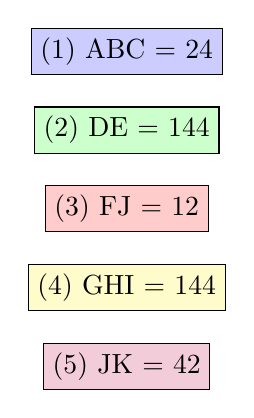
\begin{tikzpicture}
\node[draw,rectangle,fill=blue!20] at (0,4) {(1) ABC = 24};
\node[draw,rectangle,fill=green!20] at (0,3) {(2) DE = 144};
\node[draw,rectangle,fill=red!20] at (0,2) {(3) FJ = 12};
\node[draw,rectangle,fill=yellow!20] at (0,1) {(4) GHI = 144};
\node[draw,rectangle,fill=purple!20] at (0,0) {(5) JK = 42};
\end{tikzpicture}
\end{center}

\end{document}